\documentclass[12pt,a4paper]{article}
\usepackage[UKenglish]{babel} % Provides support for English ty­po­graph­i­cal and hyphen­ation rules
\usepackage[margin=2.5cm]{geometry} % Provides margins
\usepackage{unicode-math} % Provides support for fonts
\setmainfont{Junicode} % Sets font for main text
\setmathfont{Junicode} % Sets font for text in a maths environment
\setmonofont{Courier New} % Sets font for any monospaced text (e.g. URLs)
\sloppy % Relaxes rules for line breaks
%\frenchspacing % Adjusts character spacing
\linespread{1} % Adjusts line spacing
\usepackage[hidelinks]{hyperref} % Hides coloured hyperlinks
\usepackage[round]{natbib} % Provides bibliography management
\bibpunct[:]{(}{)}{,}{a}{}{,} % Sets bibliography punctuation
\setlength{\bibsep}{0em} % Gets rid of space between bibliography entries
\usepackage{sectsty} % Provides changes for sizes of section headings
\sectionfont{\normalsize} % Changes section headings to normal size
\pagestyle{empty} % Removes any content in headers and footers
\usepackage{float} % Provides options for table and figure placement
\usepackage[labelfont=bf]{caption} % Set table and figure labels to bold
\usepackage{booktabs} % Provides rules for tables
\usepackage{graphicx}
\usepackage{bibentry}
\usepackage{textcomp}
\graphicspath{ {./pictures/} }
\newcommand\email[1]{{\tt\href{mailto:#1}{#1}}} % Creates e-mail environment
\begin{document}
% Compile with XeLaTeX or LuaLaTeX and BibTeX
\raggedbottom
\begin{center}
\textbf{Don't let me be misunderstood: exploring phonological and lexical processing in auditory perception.}\\
\vspace{0.5em}
\textit{Massimiliano Canzi, The University of Manchester}\\
\vspace{0.25em}
\email{massimiliano.canzi@manchester.ac.uk}
\end{center}

\textbf{Background:} The aim of our study is to determine whether phonological information is processed earlier than semantic information in a feed-forward fashion during perception (\citealt{mcqueen2009}) or whether different levels of speech (e.g. phonological, semantic) can mediate one another during perception and processing (\citealt{mcclelland1986}). In order to achieve this, we plan to investigate the nature of early event-related potentials (ERP), shifts in electrical potential in the brain as a response to a particular event, to determine whether phonological and lexical features of speech are processed by the brain at different times. the N400 component (\citealt{kutas1980}) is a negative shift in electrical potential found approximately 400 ms post stimulus onset where the stimulus is semantically incompatible with the context in which it is found. Similarly, the phonological mismatch negativity (PMN) component (\citealt{groppe2010}) is found 200-250 ms post stimulus onset, with the stimulus being a phonologically unexpected sequence in its context (e.g. a word which begins with a phonotactically illegal syllable). This advances the idea that phonological features of speech are processed earlier in time by the brain compared to semantic features (\citealt{mcqueen2009}). However, others argue that there is little difference between N400 and pre-N400 components (\citealt{diaz2007}) and that these components are also not specific to language processing (\citealt{dikker2011}). Understanding the level of independence between N400 and pre-N400 components, together with an exploratory analysis on the language-specific nature of these components, will allow us to determine what information is processed during speech perception and when.

\textbf{Methodology:} The aim of the pilot experiment is to explore what pre-N400 effects are found in a context where an unexpected speech sequence is perceived but no lexical activation or retrieval is present. Participants are instructed to learn two pairs of trisyllabic nonce words (e.g. \textit{piputu bibapu, tapabi dipida}) where the transitional probability between the first and the second item of each pair is 1. EEG data is later recorded and the pairs of nonce words are played back to the participants of the study. However, in some cases, the first syllable of the second nonce word of each pair is manipulated to be different. Hearing unexpected phonemes should elicit pre-N400 components, which are thought to be unrelated to lexical retrieval (\citealt{groppe2010}). Future experiments will employ similar methods but different stimuli, such as real words (lexically activated) and sine-wave tones (non-speech sounds) to determine which of these components are specific to linguistic processing, if any.

\textbf{Results:} Provisional results are presented from 1 participant while more data is being collected. Figure 1 shows average electrical potential at multiple scalp sites between -200-600 ms post stimulus onset for both control and target groups, where target words contain an unexpected sequence of phonemes, different from the ones participants were previously trained on. Scalp sites include central-parietal and lateral sites where N400 and pre-N400 effects are more likely to be visible (\citealt{groppe2010}; \citealt{kutas1980}). Although more data is required in order to run any statistics on differences in mean potential amplitudes in the 200-400 ms time range between the control and target groups, scalp sites such as Cz, CP5 and CP6 show more negativity for the target condition around 200 and 400 ms, in line with findings relating to the N400 (\citealt{kutas1980}) and pre-N400 effects (\citealt{groppe2010}). Figure 2 presents a scalp map showing average electrical potential differences for the two groups between 375 and 425 ms. 

\newpage
\begin{center}
	\textbf{Figure 1:} Electrical potential (Y axis in \textmu V) for standard (freq) and odd target words between -200 and 600 ms post stimulus onset.
	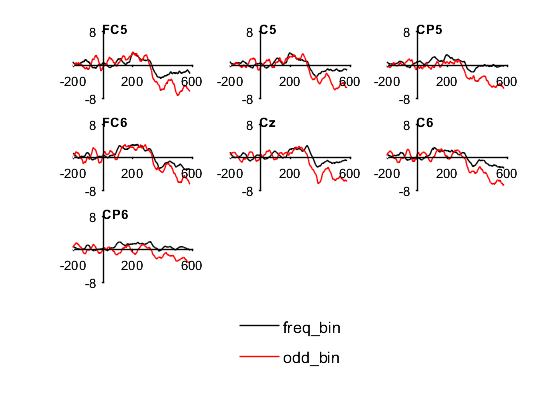
\includegraphics[scale=0.75]{waveform}
	
	\textbf{Figure 2:} Average electrical potential in \textmu V across the scalp between 375 and 425 ms for control (bin1) and target stimuli (bin2).
	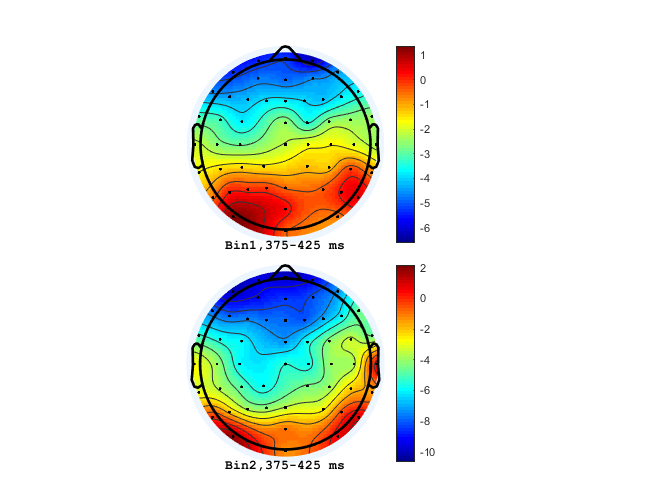
\includegraphics[scale=0.60]{map}
\end{center}

\textbf{Discussion:} The presence of the N400 component upon hearing a low-frequency nonce word, although to be confirmed by the collection of more data and the use of statistical models, could suggest that some process of lexicalisation is present for the processing of nonce words, too. This would make N400 and pre-N400 components harder to disentangle. If no N400 component is present - but pre-N400 effects are - then it would be justified to assume that pre-N400 components are in fact unrelated to semantic processing. Testing for pre-N400 components by using non-speech sounds will allows us to gather more information on the non/linguistic nature of these early ERP components. This series of experiments will allow us to address contrasting theories that, for decades, have tried to explain information flow order in speech perception.

\renewcommand\bibname{References} % Change title of bibliography from `Bibliography' to `References'
\bibliographystyle{./sp} % Specify bibliography style file
\nobibliography{./mfil.bib} % Specify bibliography file
\end{document}
